%%% LaTeX Template: Two column article
%%%
%%% Source: http://www.howtotex.com/
%%% Feel free to distribute this template, but please keep to   to http://www.howtotex.com/ here.
%%% Date: February 2011

%%% Preamble
\documentclass[landscape,	DIV=calc,%
							paper=letter,%
							fontsize=10pt,%
							twocolumn]{scrartcl}	 					% KOMA-article class

               \setlength{\columnsep}{20px}
\bibliographystyle{plain}
\makeatletter
\newcommand\notsotiny{\@setfontsize\notsotiny{6.5}{7.5}}
\makeatother
\usepackage{lipsum}													% Package to create dummy text

\usepackage[margin=.5in,footskip=0.25in]{geometry}

\usepackage[english]{babel}										% English language/hyphenation
\usepackage[protrusion=true,expansion=true]{microtype}				% Better typography
\usepackage{amsmath,amsfonts,amsthm}					% Math packages
\usepackage[pdftex]{graphicx}									% Enable pdflatex
\usepackage[svgnames,usenames,dvipsnames]{xcolor}

\usepackage[sc]{mathpazo}          % Palatino for roman (\rm)
\usepackage[scaled=0.95]{helvet}   % Helvetica for sans serif (\sf)
\usepackage{courier}               % Courier for typewriter (\tt)

\usepackage{sourcecodepro}
\usepackage[T1]{fontenc} 


\usepackage{listings} 

\definecolor{codegreen}{rgb}{0,0.9,0}
\definecolor{codegray}{rgb}{0.55,0.55,0.55}
\definecolor{codepurple}{rgb}{0.58,0,0.82}
\definecolor{backcolour}{rgb}{0.95,0.95,0.92}

\definecolor{commentgreen}{RGB}{2,112,10}
\definecolor{eminence}{RGB}{108,48,130}
\definecolor{weborange}{RGB}{255,165,0}
\definecolor{frenchplum}{RGB}{129,20,83}
\definecolor{CustomDarkRed}{RGB}{175, 0, 0} 
 

\lstdefinestyle{mystyle}{
    xleftmargin=2em,
    language=python,
    %backgroundcolor=\color{codegray},   
    commentstyle=\color{codegray},
    keywordstyle=\bfseries\color{CustomDarkRed},
    numberstyle=\tiny\color{codegray},
    stringstyle=\color{blue},
    basicstyle=\ttfamily\scriptsize,
    breakatwhitespace=false,         
    breaklines=true,                 
    captionpos=b,                    
    keepspaces=true,                 
    numbers=left,                    
    showspaces=false,                
    showstringspaces=false,
    showtabs=true,                  
    tabsize=2,
    firstnumber=last,
    mathescape=true
}

\lstset{style=mystyle}
% Enabling colors by their 'svgnames'
\usepackage[hang, small,labelfont=bf,up,textfont=it,up]{caption}	% Custom captions under/above floats
\usepackage{epstopdf}												% Converts .eps to .pdf
\usepackage{subfig}													% Subfigures
\usepackage{booktabs}												% Nicer tables
\usepackage{fix-cm}													% Custom fontsizes



%%% Custom sectioning (sectsty package)
\usepackage{sectsty}													% Custom sectioning (see below)
\allsectionsfont{%															% Change font of al section commands
	\usefont{OT1}{phv}{b}{n}%										% bch-b-n: CharterBT-Bold font
	}

\sectionfont{%																% Change font of \section command
	\usefont{OT1}{phv}{b}{n}%										% bch-b-n: CharterBT-Bold font
	}



%%% Headers and footers
\usepackage{fancyhdr}												% Needed to define custom headers/footers
	\pagestyle{fancy}														% Enabling the custom headers/footers
\usepackage{lastpage}	

% Header (empty)
\lhead{}
\chead{}
\rhead{}
% Footer (you may change this to your own needs)
\lfoot{\footnotesize \texttt{Easier AI} \textbullet ~\today}
\cfoot{}
\rfoot{\footnotesize page \thepage\ of \pageref{LastPage}}	% "Page 1 of 2"
\renewcommand{\headrulewidth}{0.0pt}
\renewcommand{\footrulewidth}{0.4pt}



%%% Creating an initial of the very first character of the content
\usepackage{lettrine}
\newcommand{\initial}[1]{%
     \lettrine[lines=3,lhang=0.3,nindent=0em]{
     				\color{DarkGoldenrod}
     				{\textsf{#1}}}{}}


\usepackage{tikz}
\definecolor{alizarin}{rgb}{0.82, 0.1, 0.26}

\newcommand*\circled[1]{\tikz[baseline=(char.base)]{
            \node[minimum width=1pt, shape=circle,fill=black,inner sep=1pt] (char) {{\footnotesize \textcolor{white}{#1}}};}}

            \newcommand{\cA}{\circled{a}}
            \newcommand{\cB}{\circled{b}}
            \newcommand{\cC}{\circled{c}}
            \newcommand{\cD}{\circled{d}}
            \newcommand{\cE}{\circled{e}}
            \newcommand{\cF}{\circled{f}}
            \newcommand{\cG}{\circled{g}}
            \newcommand{\cH}{\circled{h}}
            \newcommand{\cI}{\circled{i}}
            \newcommand{\cJ}{\circled{j}}
            \newcommand{\cK}{\circled{k}}
            \newcommand{\cL}{\circled{l}}
            \newcommand{\cM}{\circled{m}}
            \newcommand{\cN}{\circled{n}}
            \newcommand{\cO}{\circled{o}}
            \newcommand{\cP}{\circled{p}}
            \newcommand{\cQ}{\circled{q}}
            \newcommand{\cR}{\circled{r}}
            \newcommand{\cS}{\circled{s}}
            \newcommand{\cT}{\circled{t}}



%%% Title, author and date metadata
\usepackage{titling}															% For custom titles

\newcommand{\HorRule}{\color{DarkGoldenrod}%			% Creating a horizontal rule
									  	\rule{\linewidth}{1pt}%
										}
%%begin novalidate
\pretitle{\vspace{-80pt} \begin{flushleft} \HorRule 
				\fontsize{50}{50} \usefont{OT1}{phv}{b}{n} \color{DarkRed} \selectfont 
				}
    \usepackage[hidelinks]{hyperref}
\title{
    \hspace{-10mm} \begin{minipage}{.66\linewidth}
        \vspace{-25mm}Easier AI\\\Large
~\\How to  program simpler, smarter, faster, more\\\noindent
flexible and understandable analytics.~\\~\\\large
        {\em Tim Menzies + the EZR mob,  \textcolor{black}{North Carolina State University}}
    \end{minipage}
    \begin{minipage}{.28\linewidth}
        \vspace{5mm}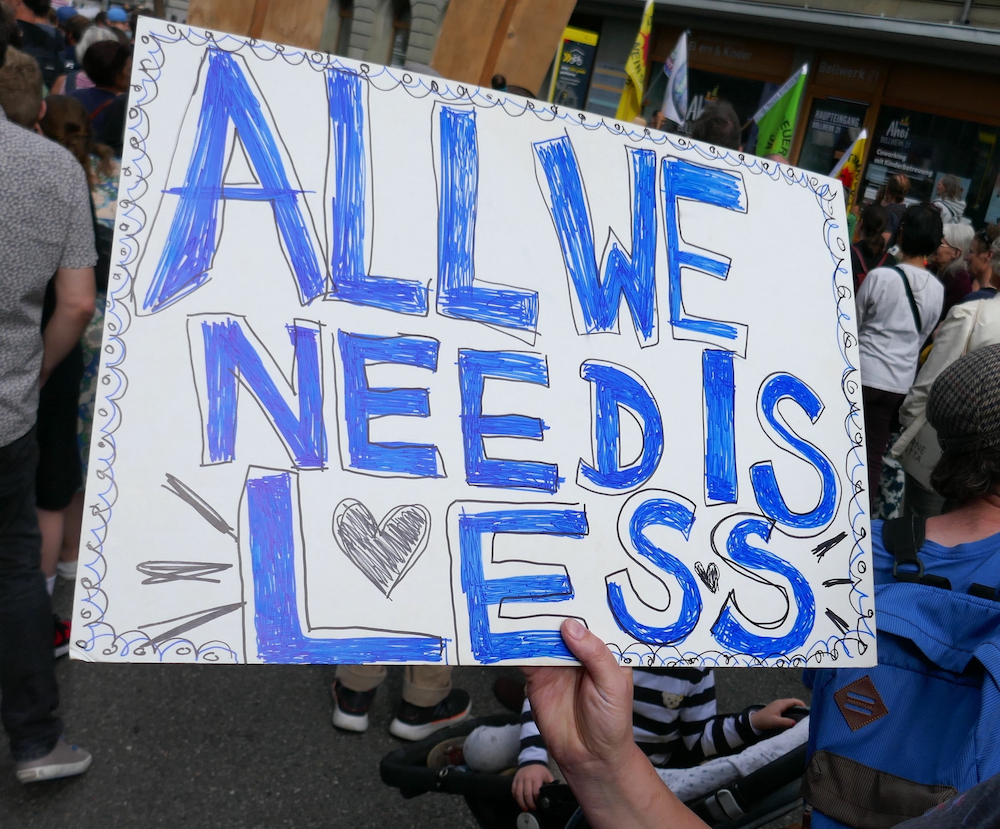
\includegraphics[width=3.2in]{Less.png}
    \end{minipage}
    }					% Title of your article goes here
\posttitle{\\\vspace{3mm} \par\end{flushleft} \vskip 0.5em}

\preauthor{\begin{flushleft}
					\large \lineskip 0.5em \usefont{OT1}{phv}{b}{sl} \color{DarkRed}}
     
\postauthor{\footnotesize \usefont{OT1}{phv}{m}{sl} 
    \vspace{-3cm} \color{Black} 
      DOI: \url{https://doi.org/10.5281/zenodo.11183059}\\
      Package: \url{https://pypi.org/project/ezr/0.1.0/}\\
      Source: \url{http://github.com/timm/ezr}\\
      Latex: \url{http://github.com/timm/ezr-tex}\\
     {\textcopyright} 2024 by Tim Menzies and the EZR mob and is licensed under \textcolor{DarkRed}{Creative Commons Attribution-ShareAlike 4.0 International}
    \LARGE ~\ccLogo  
~\ccAttribution  
~\ccShareAlike  \par\end{flushleft}\vspace{-4mm}\HorRule}
%%end novalidate
\date{}	
\usepackage{ccicons}% No date
\usepackage{enumitem}
\setlist[itemize]{noitemsep}

\newcommand{\VERSION}{3.11}

%%% Begin document
\begin{document}
\maketitle
\thispagestyle{fancy} 			% Enabling the custom headers/footers for the first page 
% The first character should be within \initial{}
\initial{A}\textbf{nalytics is how we extract high-quality insights
from low quality data. Here, we  use a ``less is more'' approach to create a
simple, fast toolkit that can tackle complex problems with just a
few data points (using incremental sampling). 
The tool supports classification, regression,
optimization, fairness, explanation, data synthesis, privacy,
compression, planning, monitoring, and runtime certification
(but not  generative tasks). 
For all these tasks, our  minimal data usage
simplifies verification.~\\~\\ 
Our message is that while not everything can be simplified,
many things can. When simplicity works, we should embrace it. Who
can argue against that?}
\subsection*{Audience}
We write this book for programmers (or those that teach programmers).
Here, we show
the most we  can do with AI, using the least amount of code.

In our own work, this material is used to teach a one semester graduate
class in SE for AI.
\subsection*{Get the code}
Our code is written in Python {\VERSION}. To install the code,
use \mbox{{\texttt pip install ezr}}. To 
        Test that installation use \mbox{{texttt ezr -h}}.


\newpage
\subsection*{About the Authors}
This book was written by the EZR mob (students from North Carolina State University, USA)
in a two-month hackathon June,July 2024. 

That work was coordinated  by Tim 
 Menzies, a professor of Computer Science at NC State University (USA).
Tim is the 
Editor-in-Chief of the
Automated Software Engineering journal; an IEEE Fellow;
and the recipient of over
over 13 million in grant money and industrial contracts.
In the literature, Google Scholar ranks him as \#2 for AI for SE and
software cost estimation, \#1 for defect prediction, and \#3 for software
analytics.  
He has graduated 50 research students-by-thesis (including 20
Ph.D.s).  This book is reversed engineered from the work of those
students, who have explored
applications of analytics for
spacecraft control, fairness, explanation, configuration, cloud computing,  security, literature reviews,
technical  debt,  vulnerability prediction, defect prediction, effort estimation,  and the management
of open source software projects.

\subsection*{Profits from this Book}
All profits from this book will be donated to the 
Direct Relief
\& Direct Relief Foundation 
(\url{https://directrelief.org}) to improve the health and lives of
people affected by poverty or emergency situations by mobilizing
and providing essential medical resources needed for their care.


\clearpage
\tableofcontents
\clearpage


\clearpage \section{Introduction: All you Need is Less}

Suppose we want to use data to make decisions about what to do,
what to avoid, what to do better, etc etc. How to do that?

This process is called {\em analytics}, i.e. the reduction of large
amounts of low-quality data into tiny high-quality statements. Think of it like
``finding the diamonds in the dust``. 
For example,
in one survey of managers at   Microsoft, 
researchers found many kinds  of analytics functions~\cite{buse2012information}.
As shown in the following table, those  functions include regression, topic analysis, anomaly detection, what-if analysis,
etc:

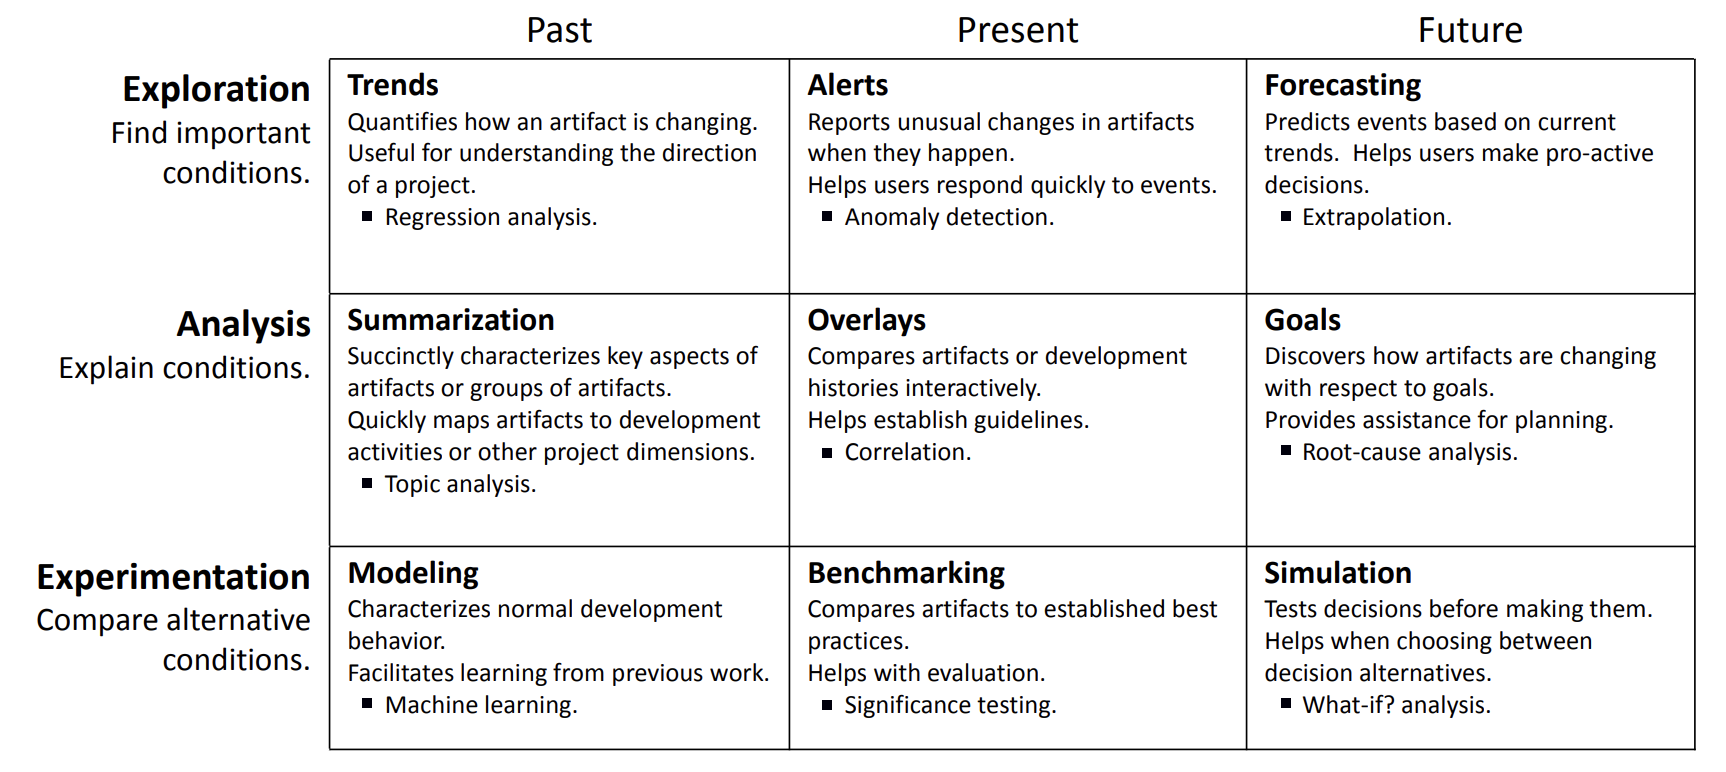
\includegraphics[width=\linewidth]{Buse.png} 

But is analytics as complicated as all that? Are all these functions really
different or do they share a
common core? And if they share a common core,
does that mean if we coded up, say, regression then everything could be coded
very quickly? 
More importantly, if we found someway to optimize
that core, would that optimization apply to many kinds of analytics?

We think so.
We've been working on applications of analytics for decades\footnote{
In that work, we've explored
data--driven applications in 
spacecraft control, fairness, explanation, configuration, cloud computing,  security, literature reviews,
technical  debt,  vulnerability prediction, defect prediction, effort estimation,  and the management
of open source software projects.}. And in all that work, one constant has been the  {\em compressability}
of the data:
\begin{itemize}
    \item
Many data sets can be pruned down to a surprisingly small set of rows and columns,
without loss of signal.
\item
In that compressed space, modeling becomes more manageable
and 
all our functions algorithms run faster (since there is less to explore).
\item
Also, 
data becomes private
since we threw away so much in the compression process.
\item
    Further,
explanation is easier since this there is less to explain. 
This means, in turn, that is easier to understand/ audit/critique
our solutions.
\end{itemize}
We are not the first to say these things.
For example, many researcher accept that higher dimensional data can often be reduced
to a
{\textbf lower dimensional latent manifolds} inside that high-dimensional
space~\cite{zhu2005semi}.
As a consequence, many data sets
that appear to initially require many variables to describe, can
actually be described by a {\textbf comparatively small number of variables}.

That said, this book has two novel features:
\begin{itemize}
    \item The simplicity of our implementation: just a few hundred  lines of Python;
    \item How much we reduce the data: often we will end up reasoning over just a few dozen key examples.
\end{itemize}
Why has not someone else published a  book showing that many seemingly complex
analytics tasks can be reduced to very simple code (that only needs a little bit of data)?
Maybe our culture prefers complex solutions:
\begin{quote}
    {\em 
Simplicity is a great virtue but it requires hard work to achieve
it and education to appreciate it. And to make matters worse:
    complexity sells better}\newline -- Edsger W. Dijkstra
\end{quote}
By making things harder than they need to be, companies can motivate
the sale  of intricate tools to clients who wished there was a
simpler way. 

Well, maybe there is a simpler way.



% This book  takes a  ``less is more'' approach to programming. 
% When the important  parts of a dozen things can be coded by one thing,
% we throw away the dozen and 
% According to  Dieter. sterwardsheip. less enrgy. 
% Code to be read at a glance (so not pep4.8a Dieter Rams'  
% ~\\
% reply: less is a bore. so if we do less we need to d more with less. more functionality. faster code. noverl results not achieved with prior approached

\newpage
% Software engineers have a superpower that lets them simplify long lists of functions
% (like the above). That superpower is called {\em refactoring}, i.e. 
% restructuring the source code  so as to improve operation.
% This document applies  refactoring to analytics. It will be seen that, under
% the hood, many
% analytics tasks share a similar set of underlying classes.  This means that
% once we code one analytics
% function, then we can quickly 
% code up many more. 

% For example, suppose we code a  DATA class that stores rows of data.
% This class:
% \begin{itemize}
%     \item
% Summarizes the columns of that data  in   NUMeric and  SYMbolic
% classes
% (one for each column);
% \item Knows how to report the expected middle values of NUMs and SYMs
%     (which is the mean or mode  for NUMs or SYMs);
% \item Knows how to report the
% diversity about that middle value (which is standard deviation or entropy for
% NUMs or SYMs).
% \end{itemize}
% This DATA class offers most of the code needed to implement  clustering  and  classification:
% \begin{itemize}
%     \item
%         A k-means clusterer picks centroids and random, then labels each row according to 
%         its nearest centroid. Those centroids are then moved to the middle of all rows with the same label and
%         the process repeats. If all the rows with the same label are stored in  a DATA class, then ``moving the centroids''
%         just means asking our NUMs and SYMs for their middle values.
% \item A Naive Bayes classifier keeps separate statistics for all the rows with the same classification.
%     If each class is implemented by a DATA class, then all those statistics can be collected just by using the DATA code.
% \end{itemize} 
% Better yet, 
% once we have a clusterer and a classifier.
%
%
%  
% the data (e.g. during a "what-if" query).  But these days, I can
% do the same analysis with 30 samples, or 
% less\footnote{Using semi-supervised multi-objective optimization via
% sequential model optimization (which is all described, later in
% this document).} 
% This means
% if someone wants to check my conclusions, they only need to review
% a few dozen samples.  Such a review was impossible using prior
% methods since the reasoning was so complicated.
%
%
% Why can I do things so easily? Well,  based on three decades of work
% on analytics~\cite{menzies1988combining} (which includes the work of 20 Ph.D. students,
% hundreds of research papers and millions of dollars in research
% funding) I say:
%
% - When building models, there are incremental methods that can find
% models after very few samples.
% - This is because the main message of most models is contained in
% just a few variables~\cite{menzies1988combining}.
%
% I'm not the first to say these things\footnote{
% From Wikipedia: The manifold hypothesis posits that many
% high-dimensional data sets that occur in the real world actually
% lie along low-dimensional latent manifolds inside that high-dimensional
% space. As a consequence of the manifold hypothesis, many data sets
% that appear to initially require many variables to describe, can
% actually be described by a comparatively small number of variables,
% likened to the local coordinate system of the underlying manifold.}.
% So it is a little
% strange that someone else has not offer something like this simpler
% synthesis. But maybe our culture prefers complex solutions:
%
% \begin{quote}{\em Simplicity is a great virtue but it requires hard work to achieve
% it and education to appreciate it. And to make matters worse:
% complexity sells better.}\newline
% -- Edger W. Dijkstra
% \end{quote}
%
% By making things harder than they need to be, companies can motivate
% the sale  of intricate tools to clients who wished there was a
% simpler way. Well, maybe there is.
%
\section{Before we Begin}
Before anything else, we need to cover some preliminaries.
\subsection{A Few Imports}
Table~\ref{tbl:create} imports the Python modules used by this code.
The line
\verb+sys.dont_write_bytecode = True+ {\cA} tells Python not
to clog the source code with a \verb+__pycahce__+ directory containing
.pyc files.

\subsection{A Few Special Types}
In this code, UPPER case words are classes and
words starting with a single upper case letter are special
types
(the special types are just used for documentation purposes and so have no methods).
For examples, as shown in Table~\ref{tbl:types}:
\begin{itemize}
    \item Missing values are marked with a \verb+DontKnow+ symbol; \cB
    \item A \verb+Row+ is a list of any atom (floats, ints, booleans, strings). {\cC} A
        \verb+Row+ can also contain \verb+DontKnow+.
    \item \verb+Rows+ hold many \verb+Row+s. {\cD}
\item \verb+Classes+ are dictionaries whose keys are class names and whose
    values are \verb+Rows+. {\cE}
\end{itemize}
Also, {\texttt OBJ} {\cF} is a handy-dandy super class for everything we do.
This class is an easy way to  generate an  {\texttt OBJ}ect with very little effort; e.g.

{\notsotiny \begin{verbatim}
person = OBJ(age=10, job="programmer")
\end{verbatim}}

\noindent
That new {\texttt OBJ}ject gives us access to all its slots for reading and update:

{\notsotiny \begin{verbatim}
person.age += 1
peron.job = "retired"
print(person)

==> OBJ{:age 11, :job retired}
\end{verbatim}}


XXXX hides slots

\newpage
\begin{table}[!h]
\begin{minipage}{\linewidth}
\begin{lstlisting}[caption={Row creation. And column header creation (from row1)},label={tbl:create}]
from __future__ import annotations   # <1> ## types  
import sys
sys.dont_write_bytecode = True $\cA$
from collections import Counter
import re,ast,copy,json,math,random
from fileinput import FileInput as file_or_stdin 
\end{lstlisting}
\end{minipage}
\end{table}

\begin{table}[!h]
\begin{minipage}{\linewidth}
\begin{lstlisting}[caption={Special types, just for this system.},label={tbl:types}]
from typing import Any,Iterable,Callable

DontKnow = "?"  $\cB$
class Row    : has:list[Any] $\cC$
class Rows   : has:list[Row] $\cD$
class Classes: has:dict[str, Rows] $\cE$

class OBJ: $\cF$
  def __init__(i,**d)    : i.__dict__.update(d)
  def __repr__(i) -> str : return i.__class__.__name__+show(i.__dict__)

def show(x:Any, n=3) -> Any:
  """Truncate long lists, round floats, recurs into dictionary values,
  do print 'secret' slots (those starting with '_')."""
  if   isinstance(x,(int,float)) : x= x if int(x)==x else round(x,n)
  elif isinstance(x,(list,tuple)): x= [show(y,n) for y in x][:10]
  elif isinstance(x,dict): 
    x= "{"+', '.join(f":{k} {show(v,n)}" for k,v in sorted(x.items()) 
                                         if k[0]!="_")+"}"
  return x
\end{lstlisting}
\end{minipage}
\end{table}

        \newpage
        \subsection{``{\texttt the}'' stores the Config }
All code has magic settings and this code is no exception.
Our config options are help in the {\texttt the} variable and is referenced
via (e.g.) {\texttt the.seed}.

\begin{table}[!h]
    \notsotiny
    \begin{verbatim}
ez.py: Active learning, find best/rest seen so far in a Bayes classifier   
(c) 2024 Tim Menzies <timm@ieee.org>, BSD-2 license   

OPTIONS:  
  -s --seed     random number seed    = 1234567891    
  -g --go       start up action       = help
  -f --file     data file             = ../data/auto93.csv    
  -n --ntiny    a tiny number         = 12   
  -N --Nsmall   a small number        = .5
    
  Discretize:
  -C --Cuts     max number divisions of numerics = 16

  Classify:     
  -k --k        low frequency kludge  = 1 
  -m --m        low frequency kludge  = 2   
    
  Optimize:    
  -i --init     initial eval budget   = 4
  -B --Budget   max eval budget       = 20
  -T --Top      keep top todos        = .8 
  
  Explain: 
  -l --leaf     min leaf size         = 2
    \end{verbatim}
\caption{Help text: defines the global options.}\label{tbl:help}
\end{table}

This {\texttt the} is generated by parsing the help string of Table~\ref{tbl:help}:
\begin{itemize}
    \item The control parameters are the word that follows ``--''.
    \item That parameter's default value is the last work on the line with ``--''.
    \item That default can be changed on the command line. E.g. our
        random number ``seed'' can be set from the Mac or UNIX operating system  
        using  \verb+ezr -s $RANDOM+
\end{itemize}

\begin{table}[!h]
\begin{minipage}{\linewidth}
\begin{lstlisting}[caption={Special types, just for this system.},label={tbl:types}]

\end{lstlisting}
\end{minipage}
\end{table}


\subsection{Just a Little Maths}
\subsubsection{Numbers and Symbols}
\subsubsection{What's in the middle? What is spread around the middle?}

\subsubsection{Pseudo-Random Numbers}

\subsection{Just a Little Stats}
\subsection{Statistically Distinguishable}
\subsection{Types}
For ease of documentation, this code uses type hints.  Most of our types are standard in Python {\VERSION}
but we had to import and define some specials:



\section{Core Classes}
How can we  combining many things into a much smaller number of things? One way is to look for
the glue, undere-the-hood, that is shared across all those things.

For analytics, that glue is the data processed by the different alorithms. So the core
of this system is 
four classes: 
\verb+DATA+, 
\verb+NUM+, 
\verb+SYM+, 
and \verb+COLS+. There are several other classes but these four are always center-stage.

\verb+DATA+ is where we store rows of data. Each column of that data is summarized
in a \verb+NUM+eric or \verb+SYM+bolic header. And \verb+COLS+ is a helper clas
that turns a list of column names into the various \verb+NUM+s and \verb+SYM+s.

\verb+DATA+ can be loaded in from file of comma-separate values. In these files,
the first row contains the column header names. For example:

{\notsotiny
\begin{verbatim}
Clndrs  Volume  Model   origin  Lbs-   Acc+  Mpg+
------  -----   ------  ------  -----  ---   ----
4       97      82      2       2130   24.6  40
4       96      72      2       2189   18    30
4       140     74      1       2542   17    30
...     ...     ....    ....    .....  .... ....
4       119     78      3       2300   14.7  30
8       260     79      1       3420   22.2  20
4       134     78      3       2515   14.8  20
6       231     78      1       3380   15.8  20
8       302     77      1       4295   14.9  20
8       351     71      1       4154   13.5  10
\end{verbatim}}
Just to explain the column names:

\begin{itemize}
    \item Names starting with ``Uppercase'' are \verb+NUM+eric and the other columns
        are \verb+SYM+bolic.  
    \item Names ending with ``-'',``+'' or ``!'' are the {\em goals}
which must  be minimized, maximized or predicted. The other columns
are the observables or controllables used to reach the goals.
\end{itemize}
The rows are all examples of some function $Y=F(X)$ where:

\begin{itemize}
    \item $Y$ are the goals (also called the dependents)
    \item $X$ are the observables or controllables (also called the independents)
    \item $F$ is the model we want to generate.
\end{itemize}
For example,  the above table is about motor cars:
\begin{itemize}
    \item
 Lighter cars cost less to build since they use less metal.
  Hence "Lbs-" (minimize weight).
\item Faster, fuel efficient cars  are easier to sell. Hence ``Acc+'' (maximize
   acceleration) and ``Mpg+'' (maximize miles per gallon).
\end{itemize}
The rows of this table are sorted by  {\em distance to heaven} i.e the
distance of each row to
some mythical best car with least weight, most acceleration and
miles per hour.  Those rows are then divided into a \verb+smallN+ best rows
(the first three rows) and rest (the other rows).

\begin{itemize}
    \item
 \verb+smallN+ is our shorthand for   $\sqrt{N}$.
\item We have another term,  \verb+tinyN+, which  denotes a dozen  ($N=12$) examples.  
\end{itemize}



\begin{table}[!t]
    \begin{lstlisting}
import re,ast
from typing import Any,Iterable,Callable
from fileinput import FileInput as file_or_stdin
#---------- ---------- ---------- ---------- ---------- ---------- ----------
def coerce(s:str) -> Any:
  "s is a int,float,bool, or a string"
  try: return ast.literal_eval(s) # 
  except Exception:  return s

def csv(file=None) -> Iterable[Row]:  $\cA$
  "read from file or standard input"
  with file_or_stdin(file) as src: 
    for line in src:
      line = re.sub(r'([\n\t\r ]|#.*)', '', line)
      if line: yield [coerce(s.strip()) for s in line.split(",")]
#---------- ---------- ---------- ---------- ---------- ---------- ----------
class COLS(OBJ): 
  """Turns a list of names into NUMs and SYMs columns. All columns are held 
  in i.all.  For convenience sake, some are also help in i.x,i.y 
  (for independent, dependent cols) as well as i.klass (for the klass goal, 
  if it exists)."""
  def __init__(i, names: list[str]): 
    i.x, i.y, i.all, i.names, i.klass = [], [], [], names, None
    for at,txt in enumerate(names):
      a,z = txt[0], txt[-1] % first and last letter
      col = (NUM if a.isupper() else SYM)(at=at,txt=txt)
      i.all.append(col)
      if z != "X": # if not ignoring, maybe make then klass,x, or y
        (i.y if z in "!+-" else i.x).append(col)
        if z == "!": i.klass= col

  def add(i,row: Row) -> Row: 
    "summarize a row into the NUMs and SYMs"
    [col.add(row[col.at]) for col in i.all if row[col.at] != "?"]
    return row
\end{lstlisting}
    \caption{Creating rows and column headers (from row1).}\label{read}
\end{table}

I'm not the first to say these things\footnote{
From Wikipedia: The manifold hypothesis posits that many
high-dimensional data sets that occur in the real world actually
lie along low-dimensional latent manifolds inside that high-dimensional
space. As a consequence of the manifold hypothesis, many data sets
that appear to initially require many variables to describe, can
actually be described by a comparatively small number of variables,
likened to the local coordinate system of the underlying manifold.}.
So it is a little
strange that someone else has not offer something like this simpler
synthesis. But maybe our culture prefers complex solutions:

\begin{quote}{\em Simplicity is a great virtue but it requires hard work to achieve
it and education to appreciate it. And to make matters worse:
complexity sells better.}\newline
-- Edsger W. Dijkstra
\end{quote}

By making things harder than they need to be, companies can motivate
the sale  of intricate tools to clients who wished there was a
simpler way. Well, maybe there is.


\clearpage
\addcontentsline{toc}{section}{References}
\bibliography{ezr.bib}
\end{document}
